\chapter{Lecture 10: Einstein's Equation, Waves, and the Cosmological Constant}

\lectureoverview{A point mass in \(2+1\) dimensions makes gravity
geometrically visible: space is a cone whose missing angle records the
mass.  From that warm-up we ask why three spatial dimensions are
special, reconstruct the conserved geometric side of Einstein's
equation, and use the equivalence principle as a practical rule for
carrying a scalar wave equation into curved spacetime.  The wave must
then gravitate in return, so we derive its stress-energy tensor and
learn why pressure and shear belong among the sources of gravity.  The
closing questions return to the cosmological constant, Einstein's
unstable static universe, light as a source, photon orbits, and the
difference between spatial flatness and flat spacetime.}

We use the signature
\begin{equation}
  g_{\mu\nu}\longrightarrow
  \eta_{\mu\nu}=\operatorname{diag}(1,-1,-1,-1)
  \label{eq:l10-signature}
\end{equation}
in a local inertial frame, and we usually set \(c=1\).  Whenever a
factor of \(c\) clarifies a physical comparison, it will be restored.

\section{A Point Mass Makes a Cone}

Begin with empty flat spacetime, and for the moment look only at a
spatial slice.  Put one point particle into an otherwise empty
\(2+1\)-dimensional universe.  The source is concentrated at one point,
so the natural question is immediate: what surface is flat everywhere
except at a single point?

\begin{classroomqa}
\audiencequestion{What geometry is flat everywhere except at the
position of the particle?
\lecturetimestamp{00:00:53--00:01:04}}
\lecturerresponse{A cone.  Cut a wedge from a flat sheet and identify
the exposed edges.  Every sufficiently small patch away from the tip is
Euclidean, yet a loop surrounding the tip detects a missing angle.  In
\(2+1\) gravity that conical defect is the exterior geometry of a point
mass.}
\end{classroomqa}

Let \(\delta\) denote the deficit angle.  The lecture needs only the
proportionality
\begin{equation}
  \delta\propto G_3 m,
  \label{eq:l10-deficit-scaling}
\end{equation}
where \(G_3\) is the Newton constant appropriate to three spacetime
dimensions.  The precise coefficient depends on convention, so the
important statement here is simpler: no mass means no missing wedge,
and increasing the mass increases the deficit.

\begin{figure}[tbp]
  \centering
  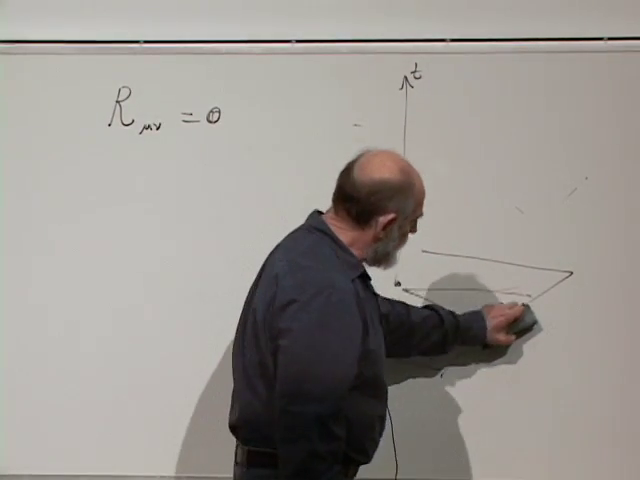
\includegraphics[width=0.84\textwidth]{lecture_10_figure_01.png}
  \caption{The conical exterior of a point source in two spatial
  dimensions.  The board sketch shows the wedge construction while
  time is understood to extend perpendicular to each conical spatial
  slice.}
  \lectureframe{00:01:45}
\end{figure}

The ideal point is not essential.  Spread the matter through a small
bounded region and the tip becomes rounded inside that region.  Outside
it, however, the geometry is still the same cone determined by the
total mass.  Thus a vacuum region can be locally flat and nevertheless
retain global information about a source enclosed by a loop.

\begin{classroomqa}
\audiencequestion{Does the deficit angle grow with the mass, and what
happens if it reaches a full turn?
\lecturetimestamp{00:01:52--00:04:29}}
\lecturerresponse{Yes.  As the missing angle approaches \(2\pi\), the
opening closes.  In the normalization used in the lecture, this occurs
when the mass reaches the scale set by the three-dimensional Planck
mass.  The humorous conclusion is also the physical one: a universe
with only two spatial dimensions leaves very little room for elaborate
gravitating structure.}
\end{classroomqa}

One spatial dimension is still more restrictive.  Three spatial
dimensions are therefore not merely an aesthetic preference; the
number of dimensions controls both the global geometry around sources
and the stability of ordinary systems.

\section{Why Three Spatial Dimensions Work}

Too few dimensions make gravity cramped.  Too many make familiar force
laws dangerously steep.  In \(d\) spatial dimensions, Gauss's law gives
the radial scaling
\begin{equation}
  F_d(r)\propto \frac{1}{r^{d-1}},
  \label{eq:l10-dimensional-force}
\end{equation}
so the familiar inverse-square law in \(d=3\) becomes inverse-cube in
\(d=4\), inverse-fourth-power in \(d=5\), and so on.

\begin{figure}[tbp]
  \centering
  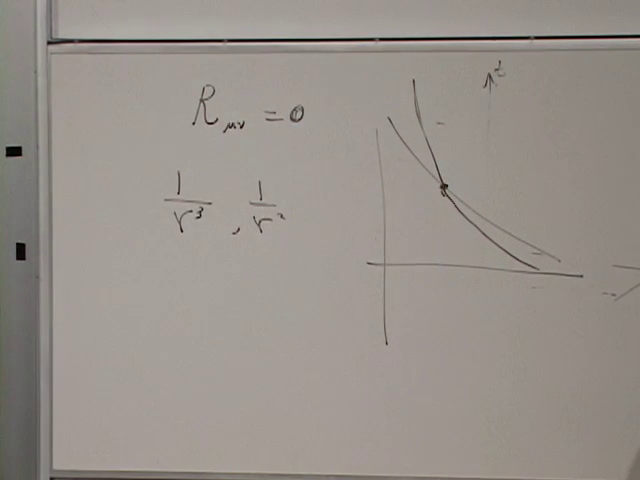
\includegraphics[width=0.88\textwidth]{lecture_10_figure_02.png}
  \caption{The board comparison of inverse-power force laws.  Relative
  to \(1/r^2\), a higher-dimensional force is weaker at large radius
  and more singular at short radius.}
  \lectureframe{00:08:00}
\end{figure}

\begin{classroomqa}
\audiencequestion{If there are more spatial dimensions, does Newton's
law remain inverse square?
\lecturetimestamp{00:05:58--00:06:14}}
\lecturerresponse{No.  The flux from a point source spreads over a
\((d-1)\)-sphere whose area grows as \(r^{d-1}\).  The force therefore
falls as \(1/r^{d-1}\).}
\end{classroomqa}

The change is fatal to the systems on which ordinary complexity
depends.  At large radius the attraction loses its grip more quickly,
so planetary orbits are not robust.  At small radius the force becomes
more singular, so an electron driven inward does not encounter the same
stable balance that exists in three dimensions.  Loosely speaking, the
outer electronic structure escapes while inner states collapse toward
the nucleus.  Without stable atoms there is no ordinary chemistry.

\begin{classroomqa}
\audiencequestion{Could nuclear forces rescue matter even if
electromagnetic atoms fail?
\lecturetimestamp{00:09:08--00:10:01}}
\lecturerresponse{They face the same dimensional problem.  Making a
short-range interaction still more singular changes the binding of
quarks and nuclei rather than preserving the hierarchy of scales we
know.  The argument is qualitative, but it shows how much of familiar
physics is tied to three spatial dimensions.}
\end{classroomqa}

\begin{classroomqa}
\audiencequestion{What about three spatial dimensions and two time
dimensions?
\lecturetimestamp{00:10:16--00:11:01}}
\lecturerresponse{That possibility is set aside rather than dressed up
as a solved problem.  Multiple time directions lead to difficult
questions about evolution, causality, and stability.  They are not
needed for the argument being developed here.}
\end{classroomqa}

No deep theorem has yet been offered that forces nature to choose
\(3+1\).  The modest conclusion is that four-dimensional spacetime is
empirically special and structurally hospitable.

\begin{classroomqa}
\audiencequestion{Why count time as a dimension at all?
\lecturetimestamp{00:11:47--00:13:23}}
\lecturerresponse{Because special relativity does not preserve a
universal split between space and time.  Lorentz boosts mix \(t\) with
a spatial coordinate, just as energy and momentum mix as components of
a four-vector.  Time is distinguished by the Lorentzian sign in
Eq.~\eqref{eq:l10-signature}, but it is not an external parameter
standing outside spacetime.  Different inertial observers choose
different time axes through the same four-dimensional geometry.}
\end{classroomqa}

\section{The Conserved Geometric Tensor}

An audience question now brings the cosmological constant into the
room.  Before asking what it does, we should see where it can enter.
The source \(T_{\mu\nu}\) is a symmetric rank-two tensor, so the
geometric side must have the same character.  From curvature, the
simplest candidates are
\begin{equation}
  R_{\mu\nu},
  \qquad
  g_{\mu\nu}R.
  \label{eq:l10-rank-two-candidates}
\end{equation}
Begin with the linear combination
\begin{equation}
  R_{\mu\nu}+C\,g_{\mu\nu}R.
  \label{eq:l10-einstein-ansatz}
\end{equation}
The coefficient is not chosen for visual symmetry.  Local
energy-momentum conservation requires
\begin{equation}
  \nabla^\mu T_{\mu\nu}=0,
  \label{eq:l10-stress-conservation}
\end{equation}
and therefore the geometric tensor equated to it must be covariantly
conserved identically.  The contracted Bianchi identity fixes
\(C=-\tfrac12\), giving
\begin{equation}
  \boxed{
  G_{\mu\nu}
  \equiv
  R_{\mu\nu}-\frac12 g_{\mu\nu}R,
  \qquad
  \nabla^\mu G_{\mu\nu}=0.}
  \label{eq:l10-einstein-tensor}
\end{equation}

\begin{figure}[tbp]
  \centering
  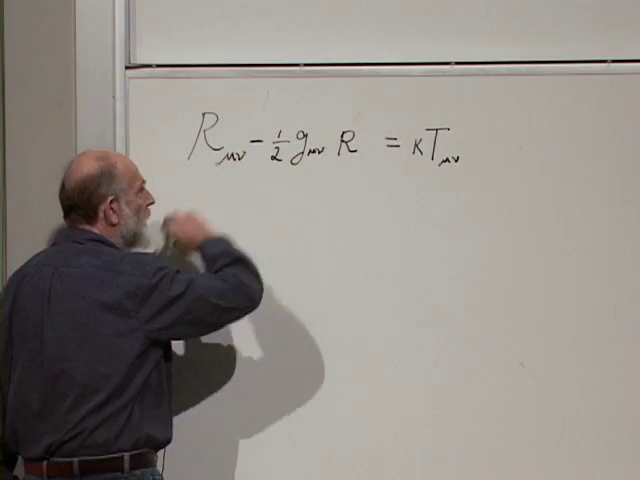
\includegraphics[width=0.88\textwidth]{lecture_10_figure_03.png}
  \caption{The Ricci tensor and scalar-curvature combination from which
  the conserved Einstein tensor is formed.}
  \lectureframe{00:16:00}
\end{figure}

\begin{figure}[tbp]
  \centering
  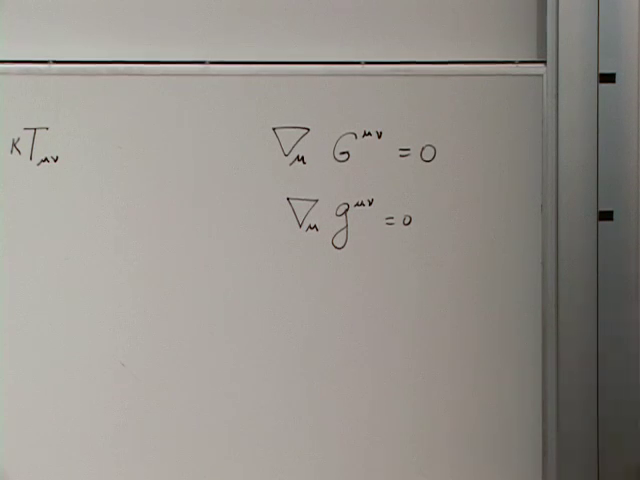
\includegraphics[width=0.72\textwidth]{lecture_10_figure_04.png}
  \caption{The two conservation identities paired on the board:
  \(\nabla_\mu G^{\mu\nu}=0\) and metric compatibility
  \(\nabla_\mu g^{\mu\nu}=0\).}
  \lectureframe{00:17:15}
\end{figure}

Metric compatibility supplies a second identically conserved
rank-two tensor:
\begin{equation}
  \nabla_\alpha g_{\mu\nu}=0.
  \label{eq:l10-metric-compatibility}
\end{equation}
Consequently a constant multiple of the metric may be added without
disturbing the conservation law.  With the standard normalization,
Einstein's equation is
\begin{equation}
  \boxed{
  G_{\mu\nu}+\Lambda g_{\mu\nu}
  =
  \frac{8\pi G}{c^4}\,T_{\mu\nu}.}
  \label{eq:l10-einstein-lambda}
\end{equation}

\begin{figure}[tbp]
  \centering
  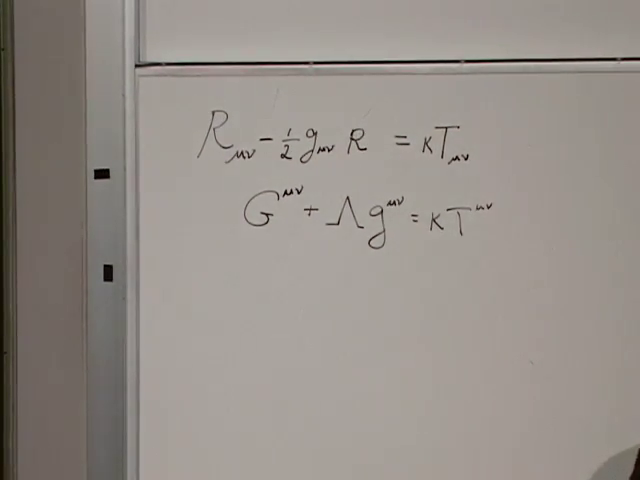
\includegraphics[width=0.84\textwidth]{lecture_10_figure_05.png}
  \caption{The cosmological term enters as a constant multiple of the
  metric, preserving the same covariant conservation law as the
  Einstein tensor.}
  \lectureframe{00:19:00}
\end{figure}

\begin{classroomqa}
\audiencequestion{Why is the covariant derivative of the metric zero?
\lecturetimestamp{00:17:05--00:18:01}}
\lecturerresponse{At any event choose local inertial coordinates.  At
that event
\[
  g_{\mu\nu}=\eta_{\mu\nu},
  \qquad
  \partial_\alpha g_{\mu\nu}=0,
\]
and the Christoffel symbols vanish.  Hence
\(\nabla_\alpha g_{\mu\nu}=0\) there.  Because the covariant derivative
of the metric is itself a tensor, vanishing in one coordinate system at
an arbitrary event means vanishing in every coordinate system at every
event.  The metric is not zero; its covariant derivative is.}
\end{classroomqa}

In the Newtonian analogy, \(\Lambda\) does not merely correct an
inverse-square law.  It creates an acceleration proportional to
distance.  Its observed value is so small that this contribution is
negligible on laboratory and planetary scales, yet it can dominate on
cosmological scales.  We postpone that consequence until the end of the
lecture.

\section{A Constrained Guess Tested Against Newton}

\begin{classroomqa}
\audiencequestion{Was Einstein's equation derived, or was it guessed
and then checked experimentally?
\lecturetimestamp{00:20:41--00:25:16}}
\lecturerresponse{It was a highly constrained physical guess.  Einstein
demanded a tensor equation with the same form in every coordinate
system, required local energy-momentum conservation, and required the
weak, static, slow-motion limit to reproduce Newtonian gravity.  Those
conditions narrow the choice dramatically, but experiment still has
the last word.}
\end{classroomqa}

To see the correspondence, write a weak static metric as
\begin{equation}
  g_{00}\simeq 1+\frac{2\Phi}{c^2},
  \qquad
  \left|\frac{\Phi}{c^2}\right|\ll 1.
  \label{eq:l10-weak-g00}
\end{equation}
For slowly moving matter, rest energy dominates:
\begin{equation}
  T_{00}\simeq \rho c^2.
  \label{eq:l10-slow-matter-t00}
\end{equation}
The \(00\)-component of Einstein's equation then reduces to the
Poisson equation
\begin{equation}
  \nabla^2\Phi=4\pi G\rho
  \label{eq:l10-poisson}
\end{equation}
when \(\Lambda\) is neglected.  Equivalently, the geometric side
contains spatial second derivatives of \(g_{00}\).  The factor of two
in Eq.~\eqref{eq:l10-weak-g00} is precisely the bookkeeping detail the
lecture warns us not to lose.

\begin{figure}[tbp]
  \centering
  
\includegraphics[width=0.84\textwidth]{lecture_10_figure_06.png}
  \caption{The \(00\)-component is reduced on the board to a
  Poisson-type equation with energy density as its source.}
  \lectureframe{00:23:15}
\end{figure}

In weak fields and at low speeds this reproduces the older theory.  At
high speeds or in strong fields the two theories differ, and the
relativistic equation is accepted because its new predictions survive
observation.  Covariance guides the guess; agreement with nature
justifies it.

\section{The Equivalence Principle as a Working Rule}

Before solving for the exterior geometry of a star, return to the
equivalence principle.  Its modern use is local and operational.  Near
any event one can choose a freely falling frame in which
\begin{equation}
  g_{\mu\nu}(P)=\eta_{\mu\nu},
  \qquad
  \partial_\alpha g_{\mu\nu}(P)=0.
  \label{eq:l10-local-inertial}
\end{equation}
Curvature, which depends on second derivatives and quadratic connection
terms, cannot in general be removed.  But over a sufficiently small
laboratory the laws of physics take their special-relativistic form.
The geographical analogy is a small patch of Earth's surface: it may
be treated as flat even though the whole surface is curved.

This gives a recipe:
\begin{enumerate}
\item write the familiar flat-spacetime law in genuine tensor form;
\item replace the flat metric by the curved metric and ordinary
derivatives by covariant derivatives where the tensor structure
requires it;
\item interpret the resulting equation locally in freely falling
frames and globally on the curved geometry.
\end{enumerate}

For a free particle, straight inertial motion becomes geodesic motion.
For the next example, use a scalar wave.

\subsection{The flat-space wave}

In one spatial dimension,
\begin{equation}
  \frac{\partial^2\phi}{\partial t^2}
  =
  c^2\frac{\partial^2\phi}{\partial x^2}.
  \label{eq:l10-wave-1d}
\end{equation}
Its general motion is assembled from profiles traveling left and
right,
\begin{equation}
  \phi(x,t)=f(x-ct)+g(x+ct),
  \label{eq:l10-wave-solutions}
\end{equation}
and linear combinations remain solutions.  In three spatial
dimensions,
\begin{equation}
  \frac{\partial^2\phi}{\partial t^2}
  =
  c^2\left(
  \frac{\partial^2\phi}{\partial x^2}
  +\frac{\partial^2\phi}{\partial y^2}
  +\frac{\partial^2\phi}{\partial z^2}
  \right).
  \label{eq:l10-wave-3d}
\end{equation}

\begin{figure}[tbp]
  \centering
  
\includegraphics[width=0.9\textwidth]{lecture_10_figure_07.png}
  \caption{The one-dimensional wave equation extended by the two
  additional spatial derivatives, with a traveling profile sketched
  at the right.}
  \lectureframe{00:34:15}
\end{figure}

Setting \(c=1\), the same equation becomes
\begin{equation}
  \eta^{\mu\nu}\partial_\mu\partial_\nu\phi=0.
  \label{eq:l10-flat-dalembert}
\end{equation}

\begin{figure}[tbp]
  \centering
  
\includegraphics[width=0.82\textwidth]{lecture_10_figure_08.png}
  \caption{The flat-space scalar wave equation written in compact
  Minkowski form beneath its component expansion.}
  \lectureframe{00:35:15}
\end{figure}

The compact notation creates a useful trap.  Replacing
\(\eta^{\mu\nu}\) by \(g^{\mu\nu}(x)\) gives an expression that looks
covariant,
\begin{equation}
  g^{\mu\nu}\partial_\mu\partial_\nu\phi,
  \label{eq:l10-naive-wave}
\end{equation}
but appearances are not enough.

\begin{classroomqa}
\audiencequestion{Why is
\(g^{\mu\nu}\partial_\mu\partial_\nu\phi=0\) not already a tensor
equation?
\lecturetimestamp{00:39:06--00:40:07}}
\lecturerresponse{The first derivative \(\partial_\nu\phi\) is a
covector because \(\phi\) is a scalar.  Raising its index produces the
vector \(g^{\mu\nu}\partial_\nu\phi\).  An ordinary derivative of that
vector is not a tensor: derivatives of the coordinate transformation
remain.  The second differentiation must therefore be covariant.}
\end{classroomqa}

The minimally coupled curved-spacetime equation is
\begin{equation}
  \boxed{
  \nabla_\mu\!\left(g^{\mu\nu}\partial_\nu\phi\right)
  =
  \nabla_\mu\nabla^\mu\phi
  =0.}
  \label{eq:l10-curved-wave}
\end{equation}
In explicit coordinates this is
\begin{equation}
  \Box_g\phi
  =
  \frac{1}{\sqrt{-g}}\,
  \partial_\mu\!\left(
  \sqrt{-g}\,g^{\mu\nu}\partial_\nu\phi
  \right)
  =0,
  \label{eq:l10-curved-wave-coordinate}
\end{equation}
where \(g=\det(g_{\mu\nu})\).

\begin{figure}[tbp]
  \centering
  
\includegraphics[width=0.92\textwidth]{lecture_10_figure_09.png}
  \caption{The curved-space wave equation written as the covariant
  divergence of the raised gradient.  The connection term appears
  because a vector is being differentiated.}
  \lectureframe{00:44:15}
\end{figure}

\begin{classroomqa}
\audiencequestion{Is general covariance by itself the whole
equivalence principle?
\lecturetimestamp{00:48:28--00:49:07}}
\lecturerresponse{No.  Covariance says that the equations retain their
tensorial meaning under a change of coordinates.  The equivalence
principle adds the physical statement that, in a sufficiently small
freely falling laboratory, nongravitational physics reduces to special
relativity.  It is this local statement that motivates the
minimal-coupling recipe.}
\end{classroomqa}

\begin{classroomqa}
\audiencequestion{Does a covariant derivative obey the ordinary
product rule?
\lecturetimestamp{00:49:13--00:51:05}}
\lecturerresponse{Yes.  It is a derivation:
\[
  \nabla_\mu(AB)=(\nabla_\mu A)B+A(\nabla_\mu B),
\]
with the appropriate index action on each factor.  Hence
\[
  \nabla_\mu(g^{\mu\nu}\partial_\nu\phi)
  =
  (\nabla_\mu g^{\mu\nu})\partial_\nu\phi
  +g^{\mu\nu}\nabla_\mu\partial_\nu\phi.
\]
Metric compatibility kills the first term and leaves
\(g^{\mu\nu}\nabla_\mu\nabla_\nu\phi\).}
\end{classroomqa}

\begin{figure}[tbp]
  \centering
  
\includegraphics[width=0.92\textwidth]{lecture_10_figure_10.png}
  \caption{The product rule and metric compatibility reduce the
  covariant divergence to the curved d'Alembertian.}
  \lectureframe{00:51:15}
\end{figure}

The metric and connection now appear as position-dependent
coefficients in the wave equation.  The analogy is a wave moving
through a medium whose density or dielectric response varies from
place to place: its propagation changes and its rays bend.  No detailed
frequency claim is needed.  The secure point is that geometry tells the
wave how to propagate.

\section{The Wave Must Gravitate in Return}

The equation \(\Box_g\phi=0\) describes one direction of the
interaction: geometry acts on the field.  General relativity requires
the reverse direction as well.  The scalar wave carries energy and
momentum, so it must supply a stress-energy tensor on the right-hand
side of Einstein's equation.

Work first in flat spacetime, where
\begin{equation}
  \Box\phi
  =
  \eta^{\mu\nu}\partial_\mu\partial_\nu\phi
  =0.
  \label{eq:l10-flat-scalar-eom}
\end{equation}
The tensor must have two indices and must be built locally from the
field.  The first derivatives provide the indexed ingredients.  A
natural ansatz is
\begin{equation}
  T_{\mu\nu}
  =
  A\,\partial_\mu\phi\,\partial_\nu\phi
  +
  C\,\eta_{\mu\nu}
  \partial_\alpha\phi\,\partial^\alpha\phi.
  \label{eq:l10-stress-ansatz-ac}
\end{equation}

\begin{classroomqa}
\audiencequestion{Why use expressions quadratic in the field rather
than terms linear in \(\phi\)?
\lecturetimestamp{00:56:50--00:59:47}}
\lecturerresponse{Changing \(\phi\) to \(-\phi\) should not reverse the
sign of the energy.  A crest and a trough, or the two sides of a
harmonic oscillation, carry the same positive energy.  The violin-string
analogy makes the same point: both velocity energy and stretching
energy are quadratic.}
\end{classroomqa}

An overall normalization can be absorbed into a rescaling of
\(\phi\), so set \(A=1\).  Conservation will determine the relative
coefficient \(C\):
\begin{equation}
  \partial^\mu T_{\mu\nu}=0.
  \label{eq:l10-flat-stress-conservation}
\end{equation}

\begin{figure}[tbp]
  \centering
  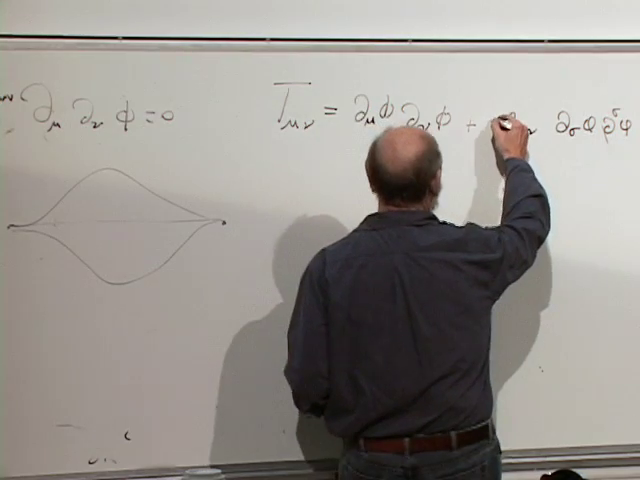
\includegraphics[width=0.92\textwidth]{lecture_10_figure_11.png}
  \caption{The quadratic scalar-field ansatz with the relative
  coefficient left undetermined.  The neighboring sketches recall
  that both signs of a wave displacement carry the same energy.}
  \lectureframe{01:00:15}
\end{figure}

\begin{classroomqa}
\audiencequestion{What does the raised index on
\(\partial^\mu\) mean?
\lecturetimestamp{01:01:10--01:02:31}}
\lecturerresponse{It is shorthand for contraction with the inverse
Minkowski metric:
\[
  \partial^\mu=\eta^{\mu\alpha}\partial_\alpha.
\]
Thus the conservation law is a four-divergence.  Raising the index
changes the signs of the spatial derivative components under the
\((+---)\) convention.}
\end{classroomqa}

Apply the product rule to the first term:
\begin{align}
  \partial^\mu
  \left(
  \partial_\mu\phi\,\partial_\nu\phi
  \right)
  &=
  (\partial^\mu\partial_\mu\phi)\partial_\nu\phi
  +
  (\partial^\mu\phi)
  (\partial_\mu\partial_\nu\phi).
  \label{eq:l10-divergence-first-term}
\end{align}
The first contribution vanishes by
Eq.~\eqref{eq:l10-flat-scalar-eom}.  For the second part of the ansatz,
\begin{align}
  \partial^\mu
  \left(
  \eta_{\mu\nu}
  \partial_\alpha\phi\,\partial^\alpha\phi
  \right)
  &=
  \partial_\nu
  \left(
  \partial_\alpha\phi\,\partial^\alpha\phi
  \right)
  \notag\\
  &=
  2(\partial^\alpha\phi)
  (\partial_\nu\partial_\alpha\phi).
  \label{eq:l10-divergence-second-term}
\end{align}
Ordinary partial derivatives commute, and the dummy index can be
renamed.  The remaining term in
Eq.~\eqref{eq:l10-divergence-first-term} therefore has exactly the same
form as one half of Eq.~\eqref{eq:l10-divergence-second-term}.

\begin{figure}[tbp]
  \centering
  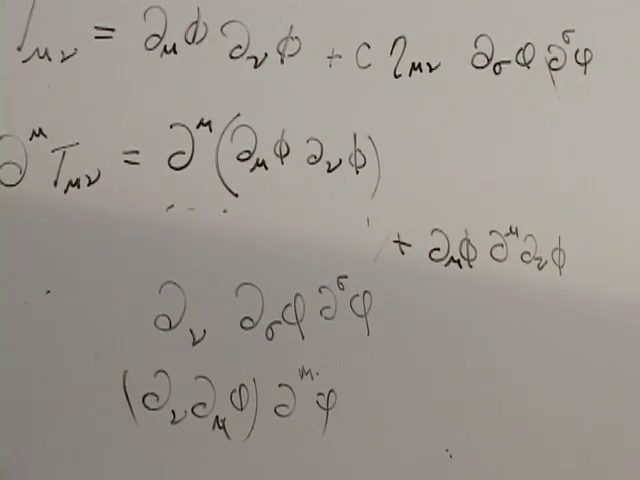
\includegraphics[width=0.92\textwidth]{lecture_10_figure_12.png}
  \caption{The product-rule calculation of
  \(\partial^\mu T_{\mu\nu}\).  One term vanishes by the wave equation;
  the two remaining derivative structures determine the relative
  coefficient.}
  \lectureframe{01:06:30}
\end{figure}

\begin{classroomqa}
\audiencequestion{Where did the first term go, and what fixes the
minus sign?
\lecturetimestamp{01:06:19--01:07:24}}
\lecturerresponse{The first term contains
\(\partial^\mu\partial_\mu\phi=\Box\phi\), so it vanishes on a solution
of the wave equation.  The surviving derivative of
\(\partial_\mu\phi\,\partial_\nu\phi\) must cancel the derivative of the
metric-proportional term.  Because the latter produces a factor of two,
conservation requires \(C=-\tfrac12\).}
\end{classroomqa}

We obtain
\begin{equation}
  \boxed{
  T_{\mu\nu}
  =
  \partial_\mu\phi\,\partial_\nu\phi
  -
  \frac12\eta_{\mu\nu}
  \partial_\alpha\phi\,\partial^\alpha\phi.}
  \label{eq:l10-scalar-stress}
\end{equation}
This is the canonical stress-energy tensor for a free massless real
scalar field in flat spacetime.

\begin{figure}[tbp]
  \centering
  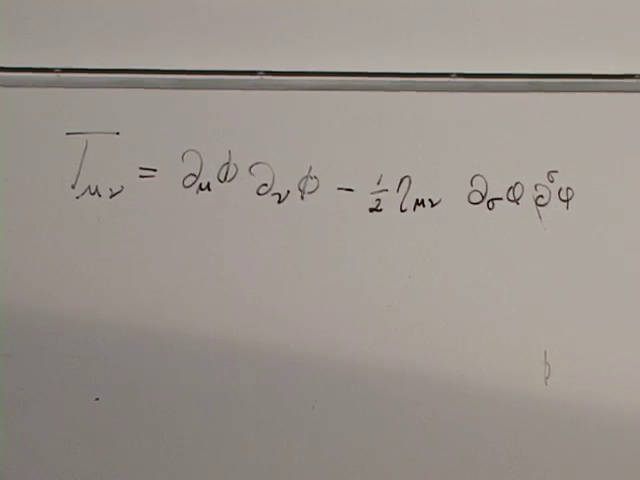
\includegraphics[width=0.92\textwidth]{lecture_10_figure_13.png}
  \caption{The completed scalar-field stress-energy tensor after the
  conservation condition fixes the coefficient \(-\tfrac12\).}
  \lectureframe{01:08:15}
\end{figure}

\subsection{Reading the energy density}

For \(\mu=\nu=0\), use
\begin{equation}
  \partial_\alpha\phi\,\partial^\alpha\phi
  =
  \dot{\phi}^{\,2}
  -
  \lvert\nabla\phi\rvert^2.
  \label{eq:l10-gradient-contraction}
\end{equation}
Then
\begin{align}
  T_{00}
  &=
  \dot{\phi}^{\,2}
  -
  \frac12
  \left(
  \dot{\phi}^{\,2}
  -
  \lvert\nabla\phi\rvert^2
  \right)
  \notag\\
  &=
  \frac12
  \left[
  \dot{\phi}^{\,2}
  +
  \left(\frac{\partial\phi}{\partial x}\right)^2
  +
  \left(\frac{\partial\phi}{\partial y}\right)^2
  +
  \left(\frac{\partial\phi}{\partial z}\right)^2
  \right].
  \label{eq:l10-scalar-energy-density}
\end{align}

\begin{classroomqa}
\audiencequestion{Does it matter whether the two zero indices are
written upstairs or downstairs?
\lecturetimestamp{01:08:05--01:08:35}}
\lecturerresponse{Not for this component in a local Minkowski frame
with \(\eta_{00}=1\): raising both zero indices introduces no sign
change.  Spatial components require more care because each raised
spatial index carries a minus sign.}
\end{classroomqa}

\begin{figure}[tbp]
  \centering
  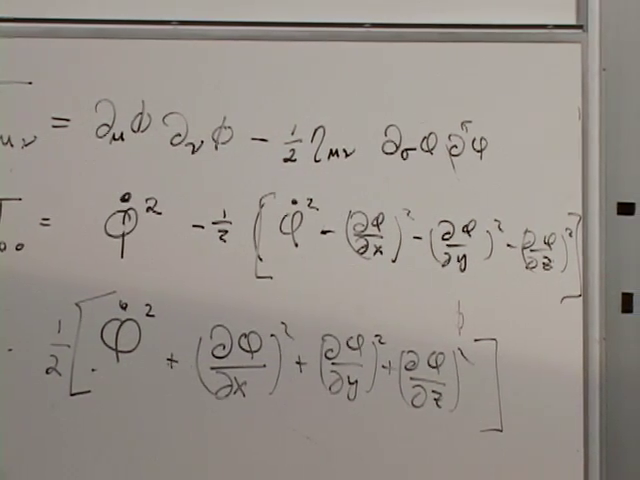
\includegraphics[width=0.94\textwidth]{lecture_10_figure_14.png}
  \caption{The stress tensor and its \(00\)-component expanded into
  kinetic energy density \(\dot{\phi}^{\,2}/2\) and gradient energy
  density \(\lvert\nabla\phi\rvert^2/2\).}
  \lectureframe{01:11:45}
\end{figure}

The two positive terms have the familiar mechanics of a vibrating
string.  Motion of the string supplies kinetic energy; spatial bending
or stretching supplies potential energy.  A wave carries both.  The
calculation has therefore done more than satisfy an index identity: it
has recovered the energy density we expected on physical grounds.

In curved spacetime the minimally coupled expression becomes
\begin{equation}
  T_{\mu\nu}
  =
  \nabla_\mu\phi\,\nabla_\nu\phi
  -
  \frac12 g_{\mu\nu}
  \nabla_\alpha\phi\,\nabla^\alpha\phi,
  \label{eq:l10-curved-scalar-stress}
\end{equation}
and it is inserted together with \(\Box_g\phi=0\) into
Eq.~\eqref{eq:l10-einstein-lambda}.  Geometry changes the wave, and the
wave's energy changes the geometry.

\section{Pressure and Shear Also Gravitate}

The phrase energy density can tempt us to look only at \(T_{00}\), but
Einstein's equation couples to the whole tensor.  In a local orthonormal
rest frame, an isotropic medium has
\begin{equation}
  T_{\hat\mu\hat\nu}
  =
  \begin{pmatrix}
    \rho & 0 & 0 & 0\\
    0 & p & 0 & 0\\
    0 & 0 & p & 0\\
    0 & 0 & 0 & p
  \end{pmatrix}.
  \label{eq:l10-perfect-fluid-covariant}
\end{equation}
With one index raised, the same convention reads
\begin{equation}
  T^{\hat\mu}{}_{\hat\nu}
  =
  \operatorname{diag}(\rho,-p,-p,-p).
  \label{eq:l10-perfect-fluid-mixed}
\end{equation}
Writing both forms prevents a common sign confusion.

\begin{figure}[tbp]
  \centering
  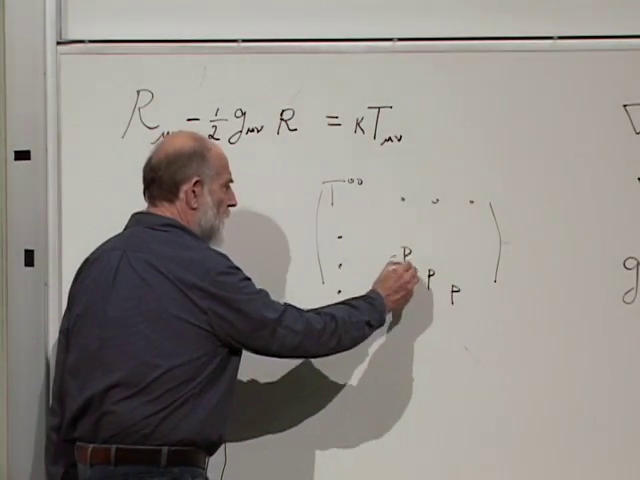
\includegraphics[width=0.86\textwidth]{lecture_10_figure_15.png}
  \caption{The isotropic rest-frame stress tensor on the board:
  energy density in the timelike slot and equal principal pressures in
  the three spatial directions.}
  \lectureframe{01:15:45}
\end{figure}

\begin{classroomqa}
\audiencequestion{Where does pressure appear in the stress-energy
tensor?
\lecturetimestamp{01:14:09--01:16:01}}
\lecturerresponse{In the spatial diagonal components in the fluid rest
frame.  For ordinary nonrelativistic matter, pressure is much smaller
than the rest-energy density \(\rho c^2\), which is why Newtonian
gravity can often ignore it.  For relativistic radiation, pressure is
of the same order as energy density; an isotropic radiation bath has
\(p=\rho/3\) when \(c=1\).}
\end{classroomqa}

Off-diagonal spatial entries describe shear stress.  Mixed time-space
entries describe momentum density or energy flux.  The tensor is
symmetric in the systems under discussion, but symmetry does not force
it to be diagonal in an arbitrary frame.

\begin{classroomqa}
\audiencequestion{Can pressure simply be added to the mass density as
one more scalar source?
\lecturetimestamp{01:18:03--01:18:39}}
\lecturerresponse{No.  Pressure can be direction-dependent, and
off-diagonal entries carry shear and momentum flux.  Rotating the axes
may diagonalize the spatial stress block, but its distinct eigenvalues
remain.  Gravity responds to the tensorial arrangement, not only to one
number called equivalent mass.}
\end{classroomqa}

The reciprocal structure can now be stated compactly:
\begin{equation}
  \begin{aligned}
    \Box_g\phi=0
    &:\quad \text{geometry}\longrightarrow\text{field propagation},
    \\
    G_{\mu\nu}+\Lambda g_{\mu\nu}
    &=8\pi G T_{\mu\nu}:\\[-0.25ex]
    &\quad \text{stress-energy}\longrightarrow\text{geometry}.
  \end{aligned}
  \label{eq:l10-reciprocal-coupling}
\end{equation}
In Wheeler's celebrated summary, matter tells spacetime how to curve,
and curved spacetime tells matter how to move.

\begin{figure}[tbp]
  \centering
  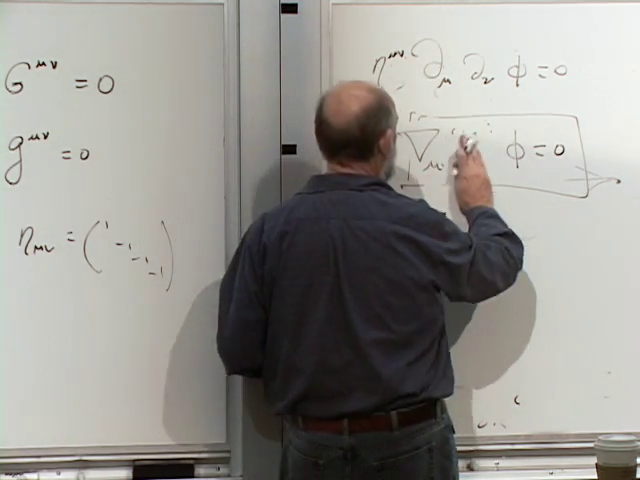
\includegraphics[width=0.88\textwidth]{lecture_10_figure_16.png}
  \caption{The two directions of the coupled system are kept together
  on the board: the wave equation contains geometry, while Einstein's
  equation contains the wave's stress-energy.}
  \lectureframe{01:19:15}
\end{figure}

\section{A Local Source Can Have a Nonlocal Field}

\begin{classroomqa}
\audiencequestion{If a mass is localized, is
\(T_{\mu\nu}\) zero everywhere else, and should the gravitational field
then vanish there?
\lecturetimestamp{01:19:44--01:22:38}}
\lecturerresponse{The stress-energy tensor may indeed vanish outside
the material body, but the field need not.  The Newtonian analogue is
Poisson's equation.  Outside a compact source,
\(\rho=0\), so \(\nabla^2\Phi=0\); nevertheless the solution
\(\Phi=-GM/r\) and its \(1/r^2\) force remain nonzero.  The source fixes
boundary data that the vacuum solution carries outward.}
\end{classroomqa}

\begin{figure}[tbp]
  \centering
  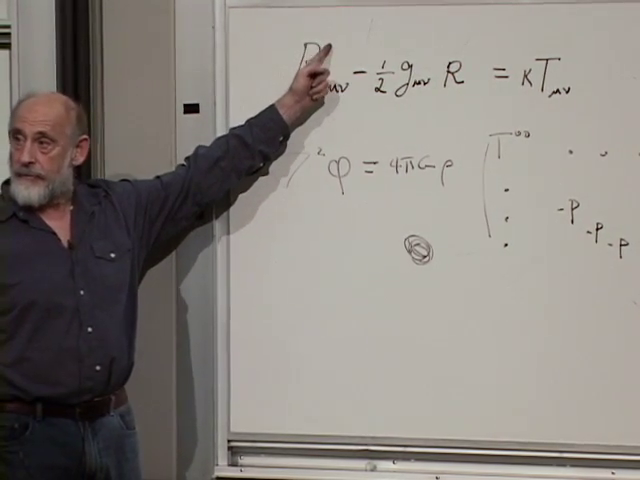
\includegraphics[width=0.9\textwidth]{lecture_10_figure_17.png}
  \caption{A localized source beside the Poisson equation.  The density
  vanishes outside the source, while the exterior potential solves the
  homogeneous equation and remains nontrivial.}
  \lectureframe{01:21:30}
\end{figure}

The relativistic version requires one refinement.  With
\(\Lambda=0\), the exterior of an isolated body can satisfy
\begin{equation}
  T_{\mu\nu}=0,
  \qquad
  R_{\mu\nu}=0,
  \label{eq:l10-vacuum-ricci}
\end{equation}
without being flat.  The full Riemann tensor may still be nonzero; its
trace-free Weyl part carries the tidal field.  Thus vacuum means
Ricci-flat here, not necessarily Riemann-flat.  This distinction is
what allows the Schwarzschild exterior to be curved even though the
matter lies inside the star.

\begin{classroomqa}
\audiencequestion{If light itself gravitates, does the superposition
principle for waves fail?
\lecturetimestamp{01:22:39--01:25:55}}
\lecturerresponse{In the coupled Einstein-field system, yes in
principle.  Two crossing or skew beams contribute stress-energy and
therefore perturb the geometry through which each beam travels.  The
effect is ordinarily fantastically small because the gravitational
mass associated with energy is \(E/c^2\).  A dimensional Newtonian
estimate for two localized energy packets gives a scale like
\[
  F_{\rm grav}\sim
  \frac{G}{r^2}\frac{E_1}{c^2}\frac{E_2}{c^2},
\]
but this is only a magnitude estimate, not a substitute for the
stress-energy of extended null beams.}
\end{classroomqa}

Linear superposition is therefore an excellent approximation for
ordinary light, not an exact principle of the full nonlinear theory.

\section{The Cosmological Constant as Long-Range Gravity}

Return now to
Eq.~\eqref{eq:l10-einstein-lambda}.  In the weak-field limit, the
cosmological constant adds a uniform term to Poisson's equation.  With
our sign convention it may be written
\begin{equation}
  \nabla^2\Phi
  =
  4\pi G\rho-\Lambda c^2.
  \label{eq:l10-poisson-lambda}
\end{equation}
In empty space, a convenient spherically symmetric solution is
\begin{equation}
  \Phi_\Lambda(r)
  =
  -\frac{\Lambda c^2}{6}r^2,
  \qquad
  \mathbf a_\Lambda
  =
  -\nabla\Phi_\Lambda
  =
  \frac{\Lambda c^2}{3}\mathbf r.
  \label{eq:l10-lambda-potential}
\end{equation}
Positive \(\Lambda\) is repulsive in this convention; negative
\(\Lambda\) is attractive.

\begin{figure}[tbp]
  \centering
  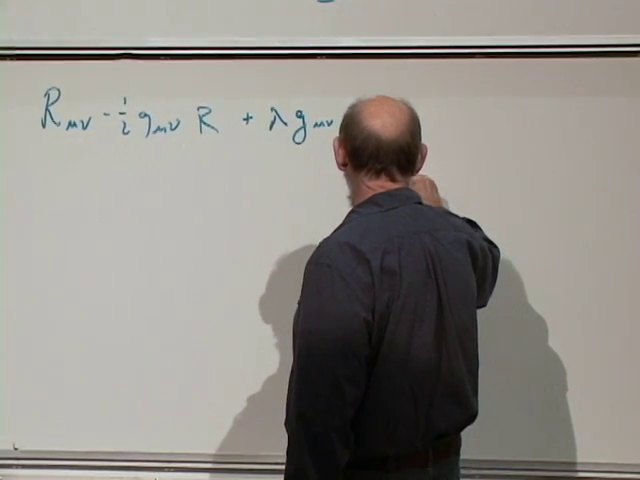
\includegraphics[width=0.9\textwidth]{lecture_10_figure_18.png}
  \caption{The Einstein equation with \(\Lambda\) and its Newtonian
  analogue: a constant source in Poisson's equation produces a
  quadratic potential.}
  \lectureframe{01:27:15}
\end{figure}

\begin{figure}[tbp]
  \centering
  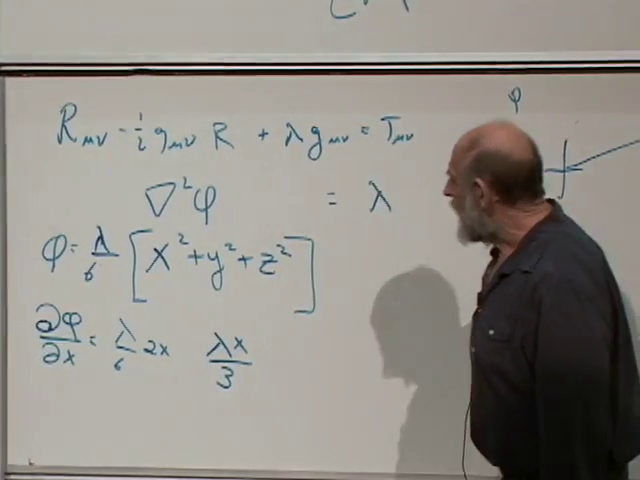
\includegraphics[width=0.88\textwidth]{lecture_10_figure_19.png}
  \caption{Differentiating the quadratic potential produces an
  acceleration linear in position.  Relative accelerations are
  homogeneous, so the construction does not select a physical center.}
  \lectureframe{01:32:15}
\end{figure}

\begin{classroomqa}
\audiencequestion{If the acceleration is proportional to distance from
an origin, does the cosmological constant pick a preferred center?
\lecturetimestamp{01:26:00--01:35:37}}
\lecturerresponse{No.  The coordinate expression uses an origin, but
the measurable statement concerns relative acceleration.  For any two
nearby points,
\[
  \mathbf a_\Lambda(\mathbf r_2)
  -
  \mathbf a_\Lambda(\mathbf r_1)
  =
  \frac{\Lambda c^2}{3}
  (\mathbf r_2-\mathbf r_1),
\]
which has the same form no matter where the coordinate origin is
placed.  A homogeneous expansion or contraction need not possess a
central point.}
\end{classroomqa}

Algebraically, \(\Lambda\) may be left with the geometry,
\begin{equation}
  G_{\mu\nu}+\Lambda g_{\mu\nu}=8\pi G T_{\mu\nu},
  \label{eq:l10-lambda-left}
\end{equation}
or moved to the matter side,
\begin{equation}
  G_{\mu\nu}
  =
  8\pi G
  \left(
  T_{\mu\nu}+T^{(\Lambda)}_{\mu\nu}
  \right),
  \qquad
  T^{(\Lambda)}_{\mu\nu}
  =
  -\frac{\Lambda}{8\pi G}g_{\mu\nu},
  \label{eq:l10-vacuum-stress}
\end{equation}
where \(c=1\).  The second notation interprets the cosmological
constant as vacuum stress-energy.  It has energy density and pressure
related by
\begin{equation}
  p_\Lambda=-\rho_\Lambda.
  \label{eq:l10-vacuum-equation-state}
\end{equation}
Whether it is written as geometry or vacuum energy, the measurable
equation is the same.

\subsection{Einstein's unstable static universe}

Historically, Einstein introduced a repulsive cosmological term to
counter the mutual attraction of matter and hold the universe static.
The cancellation can be tuned at one instant, but it is not a stable
equilibrium.

\begin{classroomqa}
\audiencequestion{Why can the cosmological constant not hold a static
universe in stable balance?
\lecturetimestamp{01:35:37--01:40:29}}
\lecturerresponse{The lecture compares the balance to a rock placed at
the top of a potential hill.  Attraction and repulsion may cancel at
one radius, but a small displacement does not produce a restoring
force.  Move slightly one way and attraction wins; move the other and
repulsion wins.  The stationary point is a maximum of the effective
potential, not a minimum.}
\end{classroomqa}

\begin{figure}[tbp]
  \centering
  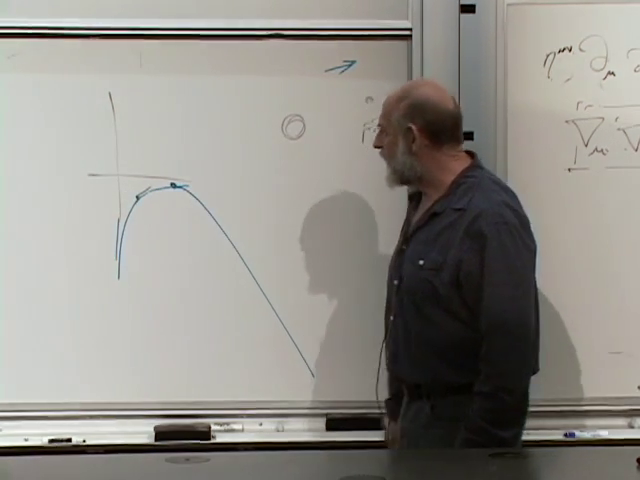
\includegraphics[width=0.8\textwidth]{lecture_10_figure_20.png}
  \caption{The effective-potential sketch for Einstein's static
  universe.  The tuned static point sits at the top of the curve and
  is therefore unstable to either contraction or expansion.}
  \lectureframe{01:39:30}
\end{figure}

The mistake was not allowing the term in the field equation.  The
mistake was expecting a delicately balanced value to make a realistic
static universe.  A small positive \(\Lambda\) remains a legitimate and
observationally important possibility.

\begin{classroomqa}
\audiencequestion{What would an attractive cosmological constant do?
Would it create a preferred origin?
\lecturetimestamp{01:40:32--01:41:23}}
\lecturerresponse{A negative \(\Lambda\) reverses the sign of the
relative acceleration and favors contraction.  It still does not
select a center: every comoving observer can describe the same
homogeneous relative motion around their own origin.}
\end{classroomqa}

\begin{classroomqa}
\audiencequestion{Could the whole universe rotate?
\lecturetimestamp{01:41:24--01:43:00}}
\lecturerresponse{No global rotation axis is observed.  A rigidly
rotating infinite universe would also force tangential speeds to grow
without bound and eventually exceed \(c\).  Local regions may rotate,
as galaxies do, but a universal rigid rotation would introduce a
preferred axis and center absent from the homogeneous picture being
discussed.}
\end{classroomqa}

\section{Principal Stresses and the Road to Schwarzschild}

The audience returns once more to the off-diagonal entries of
\(T_{\mu\nu}\).  In two spatial directions, a pure shear block may look
like
\begin{equation}
  S=
  \begin{pmatrix}
    0 & \tau\\
    \tau & 0
  \end{pmatrix}.
  \label{eq:l10-shear-block}
\end{equation}
Rotate the axes by \(45^\circ\), and the same tensor becomes
\begin{equation}
  S'=
  \begin{pmatrix}
    \tau & 0\\
    0 & -\tau
  \end{pmatrix}.
  \label{eq:l10-shear-diagonal}
\end{equation}
What appeared as shear is now compression along one principal axis and
tension along the other.

\begin{figure}[tbp]
  \centering
  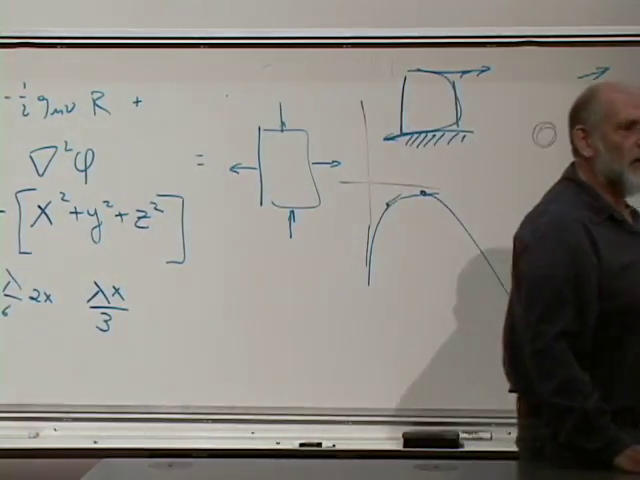
\includegraphics[width=0.92\textwidth]{lecture_10_figure_21.png}
  \caption{The shear square and its rotated principal-axis
  description.  Off-diagonal stress in one basis is unequal diagonal
  stress in another.}
  \lectureframe{01:44:45}
\end{figure}

\begin{classroomqa}
\audiencequestion{What gravitational effect should one associate with
off-diagonal stress?
\lecturetimestamp{01:43:10--01:45:37}}
\lecturerresponse{It contributes to the full spacetime geometry just
as the diagonal entries do.  Time-dependent nonspherical stresses are
among the ingredients that can generate gravitational radiation.  For
the static algebraic question, rotate to principal axes: shear becomes
unequal pressures, making its physical content easier to see.}
\end{classroomqa}

The next concrete geometry will be the exterior of a spherical mass.
Symmetry reduces the task to finding a small number of radial metric
functions, calculating their Christoffel symbols and curvature, and
solving the vacuum Einstein equations.  That solution is the
Schwarzschild metric.

\begin{classroomqa}
\audiencequestion{Can we solve intuitively for the field of a planet,
and what about a genuine two-body system?
\lecturetimestamp{01:45:37--01:47:01}}
\lecturerresponse{Spherical symmetry makes the one-body exterior
manageable and leads to Schwarzschild.  A strongly gravitating,
time-dependent two-body system has no comparable closed elementary
formula; modern calculations use numerical relativity.}
\end{classroomqa}

Light can orbit a Schwarzschild black hole, but the circular null orbit
is unstable.  If
\begin{equation}
  r_s=\frac{2GM}{c^2}
  \label{eq:l10-schwarzschild-radius}
\end{equation}
denotes the horizon radius, the photon sphere lies at
\begin{equation}
  \boxed{
  r_{\rm ph}
  =
  \frac{3GM}{c^2}
  =
  \frac32 r_s.}
  \label{eq:l10-photon-sphere}
\end{equation}
This is the corrected value previewed in the discussion: three halves
of the horizon radius, not three horizon radii.

\begin{figure}[tbp]
  \centering
  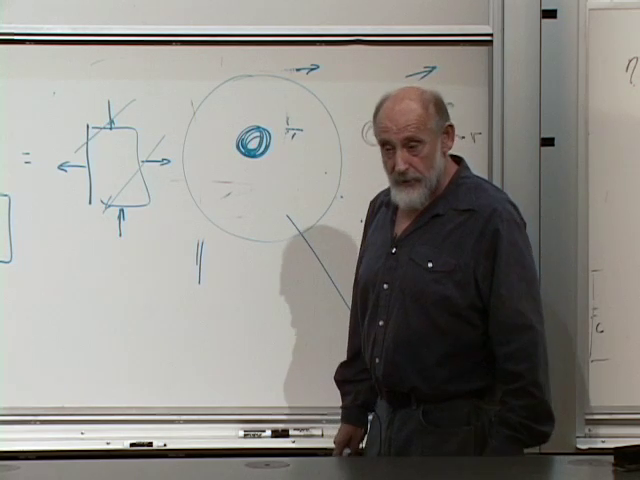
\includegraphics[width=0.88\textwidth]{lecture_10_figure_22.png}
  \caption{The board sketch of a circular light orbit around a compact
  object.  For Schwarzschild geometry the photon sphere is outside the
  horizon at \(r=3GM/c^2\), and the orbit is unstable.}
  \lectureframe{01:49:30}
\end{figure}

\begin{classroomqa}
\audiencequestion{Can enough light bind itself into a ring, and would
an observer see photons circling a black hole?
\lecturetimestamp{01:47:04--01:51:50}}
\lecturerresponse{At sufficiently high energy density, light's own
gravity cannot be ignored, although constructing a self-consistent
configuration requires the full nonlinear equations.  Around a
Schwarzschild black hole, null geodesics do admit the unstable circular
orbit of Eq.~\eqref{eq:l10-photon-sphere}.  Detailed appearance depends
on the observer and on neighboring rays, so the optical picture is
deferred until the Schwarzschild geometry is in hand.}
\end{classroomqa}

\section{Eigenvalues, Vacuum Curvature, and Two Kinds of Flatness}

At a regular material point, the stress-energy tensor can often be
understood through its eigenvectors.  In the local rest frame there is
one timelike eigenvector with eigenvalue equal to the energy density.
The three spacelike eigenvectors define principal stress directions.
Equal spatial eigenvalues give isotropic pressure; unequal ones give
anisotropic stress.

\begin{classroomqa}
\audiencequestion{What do the eigenvalues of the stress-energy tensor
mean physically?
\lecturetimestamp{01:52:02--01:53:17}}
\lecturerresponse{The timelike eigenvector identifies the comoving
frame and its eigenvalue is the rest-frame energy density.  The
spacelike eigenvalues are principal pressures.  When all three agree,
the material is isotropic; when they differ, it carries anisotropic
stress or shear.}
\end{classroomqa}

Now consider vacuum with a cosmological constant.  From
\begin{equation}
  R_{\mu\nu}
  -\frac12 g_{\mu\nu}R
  +\Lambda g_{\mu\nu}
  =0,
  \label{eq:l10-vacuum-lambda}
\end{equation}
contract with \(g^{\mu\nu}\) in four spacetime dimensions:
\begin{align}
  R-\frac12(4)R+4\Lambda&=0,
  \notag\\
  R&=4\Lambda,
  \label{eq:l10-lambda-trace}\\
  R_{\mu\nu}&=\Lambda g_{\mu\nu}.
  \label{eq:l10-lambda-ricci}
\end{align}
The sign follows the placement of \(+\Lambda g_{\mu\nu}\) in
Eq.~\eqref{eq:l10-vacuum-lambda}; moving that term or choosing the
opposite curvature convention changes intermediate signs.  The
invariant lesson is that nonzero \(\Lambda\) supports a vacuum of
constant Ricci curvature.

\begin{figure}[tbp]
  \centering
  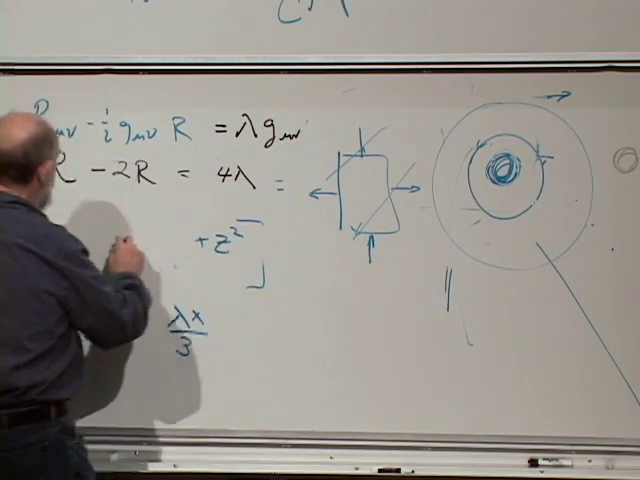
\includegraphics[width=0.92\textwidth]{lecture_10_figure_23.png}
  \caption{The vacuum Einstein equation with \(\Lambda\) and its trace
  on the board.  With the convention used here the clean result is
  \(R=4\Lambda\) and \(R_{\mu\nu}=\Lambda g_{\mu\nu}\).}
  \lectureframe{01:55:15}
\end{figure}

\begin{classroomqa}
\audiencequestion{Can an isolated system be asymptotically flat when
\(\Lambda\neq0\)?
\lecturetimestamp{01:53:30--01:56:05}}
\lecturerresponse{Not in the ordinary Minkowski sense.  For
\(\Lambda=0\), the metric of an isolated source may approach
\(\eta_{\mu\nu}\) as \(r\to\infty\).  With positive \(\Lambda\), the
vacuum approaches de Sitter behavior; with negative \(\Lambda\), it
approaches anti-de Sitter behavior.  The cosmological term eventually
dominates over the localized source.}
\end{classroomqa}

\begin{classroomqa}
\audiencequestion{Can a universe with a cosmological constant be
spatially finite?
\lecturetimestamp{01:56:05--01:56:39}}
\lecturerresponse{Yes.  Closed spatial geometries are possible, but
finiteness is not determined by \(\Lambda\) alone.  Matter content,
initial conditions, and the chosen cosmological solution all enter.
The detailed classification belongs to cosmology.}
\end{classroomqa}

\begin{classroomqa}
\audiencequestion{When we say the universe is flat, do we mean that
spacetime is flat?
\lecturetimestamp{01:56:41--01:58:29}}
\lecturerresponse{Not necessarily.  Cosmologists often say that a
constant-time spatial slice has nearly zero intrinsic curvature.
Spacetime can still be curved because the scale factor evolves and
because matter or \(\Lambda\) is present.  By contrast, asymptotic
flatness for an isolated system means that the full spacetime metric
approaches the Minkowski metric far from the source.}
\end{classroomqa}

\section{What Has Been Assembled}

The lecture began with a cone because it is the cleanest example of
geometry remembering a source.  It then enlarged that lesson in three
directions.

\begin{enumerate}
\item Conservation selects the Einstein tensor but still permits the
cosmological term:
\[
  G_{\mu\nu}+\Lambda g_{\mu\nu}
  =
  \frac{8\pi G}{c^4}T_{\mu\nu}.
\]
\item The equivalence principle turns special relativity into a
construction rule.  For a scalar wave it yields
\[
  \Box_g\phi=0.
\]
\item The wave carries the conserved stress-energy
\[
  T_{\mu\nu}
  =
  \nabla_\mu\phi\,\nabla_\nu\phi
  -
  \frac12 g_{\mu\nu}
  \nabla_\alpha\phi\,\nabla^\alpha\phi,
\]
so the field and geometry must be solved together.
\end{enumerate}

Mass density is only the first entry in the source tensor.  Momentum,
pressure, shear, radiation, and vacuum energy all gravitate.  Vacuum
outside matter need not be flat, and a nonzero cosmological constant
changes the very notion of the distant vacuum.  With that structure in
place, the next lecture can stop speaking abstractly and solve the
first central example: the Schwarzschild geometry of a spherical mass,
with cosmological expansion waiting just beyond it.
